% -*- coding: utf-8 -*-
%-------------------------designed by zcf--------------
\documentclass[UTF8,a4paper,10pt]{ctexart}
\usepackage[left=3.17cm, right=3.17cm, top=2.74cm, bottom=2.74cm]{geometry}
\usepackage{amsmath}
\usepackage{graphicx,subfig}
\usepackage{float}
\usepackage{cite}
\usepackage{caption}
\usepackage{enumerate}
\usepackage{booktabs} %表格
\usepackage{multirow}
\usepackage{pythonhighlight}
\newcommand{\tabincell}[2]{\begin{tabular}{@{}#1@{}}#2\end{tabular}}  %表格强制换行
%-------------------------字体设置--------------
\usepackage{times} 
\newcommand{\yihao}{\fontsize{26pt}{36pt}\selectfont}           % 一号, 1.4 倍行距
\newcommand{\erhao}{\fontsize{22pt}{28pt}\selectfont}          % 二号, 1.25倍行距
\newcommand{\xiaoer}{\fontsize{18pt}{18pt}\selectfont}          % 小二, 单倍行距
\newcommand{\sanhao}{\fontsize{16pt}{24pt}\selectfont}  %三号字
\newcommand{\xiaosan}{\fontsize{15pt}{22pt}\selectfont}        % 小三, 1.5倍行距
\newcommand{\sihao}{\fontsize{14pt}{21pt}\selectfont}            % 四号, 1.5 倍行距
\newcommand{\banxiaosi}{\fontsize{13pt}{19.5pt}\selectfont}    % 半小四, 1.5倍行距
\newcommand{\xiaosi}{\fontsize{12pt}{18pt}\selectfont}            % 小四, 1.5倍行距
\newcommand{\dawuhao}{\fontsize{11pt}{11pt}\selectfont}       % 大五号, 单倍行距
\newcommand{\wuhao}{\fontsize{10.5pt}{15.75pt}\selectfont}    % 五号, 单倍行距
%-------------------------章节名----------------
\usepackage{ctexcap} 
\CTEXsetup[name={,、},number={ \chinese{section}}]{section}
\CTEXsetup[name={(,)},number={\chinese{subsection}}]{subsection}
\CTEXsetup[name={,.},number={\arabic{subsubsection}}]{subsubsection}
%-------------------------页眉页脚--------------
\usepackage{fancyhdr}
\pagestyle{fancy}
\lhead{\kaishu \leftmark}
% \chead{}
\rhead{\kaishu 机器学习实验报告}%加粗\bfseries 
\lfoot{}
\cfoot{\thepage}
\rfoot{}
\renewcommand{\headrulewidth}{0.1pt}  
\renewcommand{\footrulewidth}{0pt}%去掉横线
\newcommand{\HRule}{\rule{\linewidth}{0.5mm}}%标题横线
\newcommand{\HRulegrossa}{\rule{\linewidth}{1.2mm}}
%-----------------------伪代码------------------
\usepackage{algorithm}  
\usepackage{algorithmicx}  
\usepackage{algpseudocode}  
\floatname{algorithm}{Algorithm}  
\renewcommand{\algorithmicrequire}{\textbf{Input:}}  
\renewcommand{\algorithmicensure}{\textbf{Output:}} 
\usepackage{lipsum}  
\makeatletter
\newenvironment{breakablealgorithm}
  {% \begin{breakablealgorithm}
  \begin{center}
     \refstepcounter{algorithm}% New algorithm
     \hrule height.8pt depth0pt \kern2pt% \@fs@pre for \@fs@ruled
     \renewcommand{\caption}[2][\relax]{% Make a new \caption
      {\raggedright\textbf{\ALG@name~\thealgorithm} ##2\par}%
      \ifx\relax##1\relax % #1 is \relax
         \addcontentsline{loa}{algorithm}{\protect\numberline{\thealgorithm}##2}%
      \else % #1 is not \relax
         \addcontentsline{loa}{algorithm}{\protect\numberline{\thealgorithm}##1}%
      \fi
      \kern2pt\hrule\kern2pt
     }
  }{% \end{breakablealgorithm}
     \kern2pt\hrule\relax% \@fs@post for \@fs@ruled
  \end{center}
  }
\makeatother
%------------------------代码-------------------
\usepackage{xcolor} 
\usepackage{listings} 
\lstset{ 
breaklines,%自动换行
basicstyle=\small,
escapeinside=``,
keywordstyle=\color{ blue!70} \bfseries,
commentstyle=\color{red!50!green!50!blue!50},% 
stringstyle=\ttfamily,% 
extendedchars=false,% 
linewidth=\textwidth,% 
numbers=left,% 
numberstyle=\tiny \color{blue!50},% 
frame=trbl% 
rulesepcolor= \color{ red!20!green!20!blue!20} 
}
%------------超链接----------
\usepackage[colorlinks,linkcolor=black,anchorcolor=blue]{hyperref}
%------------------------TODO-------------------
\usepackage{enumitem,amssymb}
\newlist{todolist}{itemize}{2}
\setlist[todolist]{label=$\square$}
% for check symbol 
\usepackage{pifont}
\newcommand{\cmark}{\ding{51}}%
\newcommand{\xmark}{\ding{55}}%
\newcommand{\done}{\rlap{$\square$}{\raisebox{2pt}{\large\hspace{1pt}\cmark}}\hspace{-2.5pt}}
\newcommand{\wontfix}{\rlap{$\square$}{\large\hspace{1pt}\xmark}}
%------------------------水印-------------------
\usepackage{tikz}
\usepackage{xcolor}
\usepackage{eso-pic}

\newcommand{\watermark}[3]{\AddToShipoutPictureBG{
\parbox[b][\paperheight]{\paperwidth}{
\vfill%
\centering%
\tikz[remember picture, overlay]%
  \node [rotate = #1, scale = #2] at (current page.center)%
    {\textcolor{gray!80!cyan!30!magenta!30}{#3}};
\vfill}}}



%———————————————————————————————————————————正文———————————————————————————————————————————————
%----------------------------------------------
\begin{document}
\begin{titlepage}
    \begin{center}
    
\includegraphics[width=0.8\textwidth]{NKU.png}\\[1cm]    
    \textsc{\Huge \kaishu{\textbf{南\ \ \ \ \ \ 开\ \ \ \ \ \ 大\ \ \ \ \ \ 学}} }\\[0.9cm]
    \textsc{\huge \kaishu{\textbf{计\ \ 算\ \ 机\ \ 学\ \ 院}}}\\[0.5cm]
    \textsc{\Large \textbf{机器学习实验报告}}\\[0.8cm]
    \HRule \\[0.9cm]
    { \LARGE \bfseries 实验三\ 参数估计与非参数估计}\\[0.4cm]
    \HRule \\[2.0cm]
    \centering
    \textsc{\LARGE \kaishu{姓名\ :\ 王泳鑫}}\\[0.5cm]
    \textsc{\LARGE \kaishu{学号\ :\ 1911479}}\\[0.5cm]
    \textsc{\LARGE \kaishu{年级\ :\ 2019级}}\\[0.5cm]
    \textsc{\LARGE \kaishu{专业\ :\ 计算机科学与技术}}\\[0.5cm]
    \textsc{\LARGE \kaishu{指导教师\ :\ 卫金茂}}\\[0.5cm]
    \vfill
    {\Large \today}
    \end{center}
\end{titlepage}
%-------------摘------要--------------
\newpage
\thispagestyle{empty}
\renewcommand{\abstractname}{\kaishu \sihao \textbf{摘要}}
    \begin{abstract}

        \noindent  %顶格
        \textbf{\\\ 关键字:参数估计,Machine Learning , Deep Learning}\textbf{} \\\ \\\
    \end{abstract}
%----------------------------------------------------------------
\tableofcontents
%----------------------------------------------------------------
\newpage
\watermark{60}{10}{NKU}
\setcounter{page}{1}
%——————————————————————————————————————
\section{实验描述}
\subsection{实验内容}

\subsection{实验要求}
基本要求:

在两个数据集应用“最大后验概率规则”进行分类实验,计算分类错误率,分析实验结果。

中级要求:

在两个数据集合上使用高斯核函数估计方法,应用“似然率测试规则”分类,在[0.1,0.5,1,1.5,2]范围内交叉验证找到最优h值,分析实验结果。
%——————————————————————————————————————
\section{代码实现}

\subsection{基本要求}
首先,这次实验没有给出数据集,而是需要我们利用np.random.multivariate\_normal(mean, cov, temp\_num)函数来生成随机数据,这些数据符合正态分布,
生成两个各包含 $\mathrm{N}=1000$ 个二维随机矢量的数据集合 $X_{1}$ 和 $X_{2}$, 数据集合中随机矢量 来自于三个分布模型, 分别满足均值矢量 $\mathbf{m}_{1}=[1,1]^{T}, \mathbf{m}_{2}=[4,4]^{T}, \mathbf{m}_{3}=[8,1]^{T}$ T和协方差矩 阵 $\mathbf{S}_{1}=\mathbf{S}_{2}=\mathbf{S}_{3}=2 \mathbf{I}$, 其中 $\mathbf{I}$ 是 $2 \times 2$ 的单位矩阵。在生成数据集合 $\mathrm{X}$ 时, 假设来自三个 分布模型的先验概率相同 $p\left(w_{1}\right)=p\left(w_{2}\right)=p\left(w_{3}\right)=1 / 3$; 而在生成数据集合 $\mathrm{X}$ ' 时, 先验 概率分别为 $p\left(w_{1}\right)=0.6, p\left(w_{2}\right)=0.3, p\left(w_{3}\right)=0.1$ 。代码如下:

\begin{python}
def generate_dataset():
   m1 = (1, 1)
   m2 = (4, 4)
   m3 = (8, 1)

   s1 = s2 = s3 = [[2, 0], [0, 2]]
   x1 = []
   x2 = []

   for i in range(333):
       x1.append(np.random.multivariate_normal(m1, s1))
       x1.append(np.random.multivariate_normal(m2, s2))
       x1.append(np.random.multivariate_normal(m3, s3))
   x1.append(np.random.multivariate_normal(m1, s1))
   for i in range(600):
       x2.append(np.random.multivariate_normal(m1, s1))

   for i in range(300):
       x2.append(np.random.multivariate_normal(m1, s1))

   for i in range(100):
       x2.append(np.random.multivariate_normal(m1, s1))

   x1 = np.array(x1)
   x2 = np.array(x2)
   return x1, x2

\end{python}

然后我们要对行训练集与验证集的划分,与前两次实验一样,我们仍旧采用多折交叉验证的方式。需
注意的是,为保证验证集中各类数据出现概率均等,我们需要先把 3 类数据分开
后再分别划分训练集和测试集:

\begin{python}
   def train_valid_split(data, label, fold, idx):
    sample1 = data[:333]
    label1 = label[:333]
    sample2 = data[333:666]
    label2 = label[333:666]
    sample3 = data[666:]
    label3 = label[666:]
    train_idx = []
    valid_sample = []
    valid_label = []
    for i in range(sample1.shape[0]):
        if i%fold == idx:
            valid_sample.append(sample1[i, :])
            valid_sample.append(sample2[i, :])
            valid_sample.append(sample3[i, :])
            valid_label.append(label1[i])
            valid_label.append(label2[i])
            valid_label.append(label3[i])
        else:
            train_idx.append(i)
    train_sample1 = sample1[train_idx, :]
    train_sample2 = sample2[train_idx, :]
    train_sample3 = sample3[train_idx, :]
    train_label1 = label1[train_idx]
    train_label2 = label2[train_idx]
    train_label3 = label3[train_idx]
    valid_sample = np.array(valid_sample)
    valid_label = np.array(valid_label)
    return train_sample1, train_sample2, train_sample3, \
           train_label1, train_label2, train_label3, \
           valid_sample, valid_label
\end{python}

然后我们便可开始参数估计的核心内容了,首先我们进行正态分布条件下的
参数估计。根据前文分析得到的参数计算公式,定义参数计算函数为:

\begin{python}
   def cal_para(sample):
    dim = sample.shape[1]
    mean = np.mean(sample, 0)
    sigma = np.cov(sample.T)
    det_sigma = np.linalg.det(sigma)
    return dim, mean, sigma, det_sigma
\end{python}

得到概率密度函数中的各参数后,我们构造概率密度函数公式,定义概率计
算函数为:

\begin{python}
   def cal_prob(vec, sample):
    dim, mean, sigma, det_sigma = cal_para(sample)
    # 正态分布概率密度函数
    prob = (1 / (((2*np.pi) ** (dim/2)) * np.sqrt(det_sigma))) * \
           np.exp((-(1/2) * (vec - mean)).dot(np.mat(sigma).I).dot(vec - mean))
    return prob
\end{python}

得到概率值后,我们基于实验要求中的似然概率测试规则,比较验证集中各
条样本对应的 3 类分布的概率大小,将概率值最大的 1 类作为验证样本的预测标
签:

\begin{python}
   def pred_label(valid, train_sample1, train_sample2, train_sample3):
    label = []
    for i in range(valid.shape[0]):
        prob1 = cal_prob(valid[i, :], train_sample1)
        prob2 = cal_prob(valid[i, :], train_sample2)
        prob3 = cal_prob(valid[i, :], train_sample3)
        if max([prob1, prob2, prob3]) == prob1:  # 选择概率值最大的作为预测标签
            label.append(1)
        elif max([prob1, prob2, prob3]) == prob2:
            label.append(2)
        else:
            label.append(3)
    return np.array(label)

\end{python}

最后再通过交叉检验得到正确率:

\begin{python}
   def cross_valid(data, label, fold):
    acc = []
    for i in range(fold):
        train_sample1, train_sample2, train_sample3, \
        train_label1, train_label2, train_label3, \
        valid_sample, valid_label = train_valid_split(data, label, fold, i)
        pred = pred_label(valid_sample, train_sample1, train_sample2,train_sample3)
        correct = 0
        for j in range(valid_label.shape[0]):
            if pred[j] == valid_label[j]:
                correct += 1
        print(i, 'acc', correct/valid_label.shape[0])
        acc.append(correct/valid_label.shape[0])
    return np.mean(acc)
\end{python}


\subsection{提高要求}

对于选取最合适h的大小,我们可以通过sklearn库中kde.KernelDensity来改变,再通过最大似然概率,选取标签,代码如下(大致与要求1相同):

\begin{python}
   def cal_prob_smooth(vec, sample,h):
    model = kde.KernelDensity(kernel='gaussian', bandwidth=h).fit(sample)
    prob = np.exp(model.score_samples(vec.reshape(1, -1)))
    return prob

\end{python}

最后仍是通过交叉检验得到平均的准确率,在不同的h值下,平均的准确率也不同:

\begin{python}
   def cross_valid(data, label, fold,h):
    acc = []
    for i in range(fold):
        train_sample1, train_sample2, train_sample3, \
        train_label1, train_label2, train_label3, \
        valid_sample, valid_label = train_valid_split(data, label, fold, i)
        pred = pred_label(valid_sample, train_sample1, train_sample2,train_sample3,h)
        correct = 0
        for j in range(valid_label.shape[0]):
            if pred[j] == valid_label[j]:
                correct += 1
        ##print(h,"   ",i, 'acc', correct/valid_label.shape[0])
        acc.append(correct/valid_label.shape[0])

    print("when h is ",h," , the acc is",np.mean(acc))
    return np.mean(acc)

\end{python}
%——————————————————————————————————————
\section{实验结果展示与分析}

\subsection{实验结果1}
实验结果如图\ref{fig:1}所示
\begin{figure}[H]
    \centering
    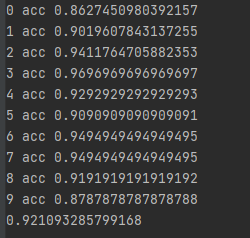
\includegraphics[scale=0.7]{1.png}
    \caption{交叉验证结果}
    \label{fig:1}
\end{figure}

\subsection{实验结果2}

实验结果如图\ref{fig:1}所示
\begin{figure}[H]
    \centering
    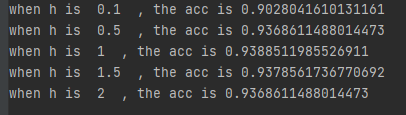
\includegraphics[scale=0.7]{2.png}
    \caption{交叉验证结果}
    \label{fig:1}
\end{figure}

我们可以看到对于随机生成数据集来说,h在[0.5,1,1.5,2]这几个h值下,准确率都比较高,但是当h为1时,
平均准确率最高,达到0.93885。

%----------------------------------------------------------------

%----------------------------------------------------------------
\bibliographystyle{plain}
\end{document}
